\documentclass[12pt, oneside]{report}

\usepackage[left=2.5cm, top=2.5cm, bottom=2.5cm, right=2.5cm]{geometry}

\usepackage[backend=bibtex,style=verbose-trad2]{biblatex}
\bibliography{bibliography}

\usepackage[utf8]{inputenc}
\usepackage[T1]{polski}
\usepackage[polish,english]{babel}
\selectlanguage{polish}
\usepackage{svg}
\usepackage{pdfpages}
\usepackage{subcaption}

\begin{document}
\thispagestyle{empty}
\begin{titlepage}
    \begin{center}

           \Large
	\textbf{Uniwersytet Jagielloński w Krakowie}\vspace{0.2cm}\\ Wydział Fizyki, Astronomii i Informatyki Stosowanej
               \vspace*{1cm}

         \vspace{3cm}
         \Large
          \textbf{Jakub Wida}\\\vspace{0.5cm}
         \normalsize Nr albumu: 1113470\\
             \vspace{2cm}
        \Huge
        \textbf{Losowe upakowania układów złożonych z dysków z wykorzystaniem kart graficznych}

        \vspace{1.5cm}
        \normalsize
        Praca magisterska\\
        na kierunku Informatyka Stosowana\\ \vspace{0.15cm}

        \vfill
        \vspace{2cm}
       \begin{minipage}{1\textwidth}
\begin{flushright}
Praca wykonana pod kierunkiem\\
dr. hab. Michała Cieśli\\
z Zakładu Fizyki Statystycznej
\end{flushright}
\end{minipage}

        \vspace{2cm}
        \begin{center}
      Kraków 2019
        \end{center}
    \end{center}
\end{titlepage}

\newpage
 \thispagestyle{empty}
\vspace{2.5cm}
\begin{flushleft}
\large \textbf{Oświadczenie autora pracy}\vspace{0.6cm}\\
\end{flushleft}

\noindent Świadom odpowiedzialności prawnej oświadczam, że niniejsza praca dyplomowa została napisana przeze mnie samodzielnie i nie zawiera treści uzyskanych w sposób niezgodny z obowiązującymi przepisami.\\

\noindent Oświadczam również, że przedstawiona praca nie była wcześniej przedmiotem procedur związanych z uzyskaniem tytułu zawodowego w wyższej uczelni.
\vspace{2cm}
\begin{center}
\begin{tabular}{lr}
................................~~~~~~~~~~~~~~~~~~~~~~~~~~~~~~~~~~~~~~&
.......................................... \\
{~~~~Kraków, dnia} & {Podpis autora pracy~~~~}
\end{tabular}
\end{center}
\vspace{5cm}
\begin{flushleft}
\large \textbf{Oświadczenie kierującego pracą}
\end{flushleft}

\noindent Potwierdzam, że niniejsza praca została przygotowana pod moim kierunkiem i~kwalifikuje się do przedstawienia jej w postępowaniu o nadanie tytułu zawodowego.
\vspace{2cm}
\begin{center}
\begin{tabular}{lr}
................................~~~~~~~~~~~~~~~~~~~~~~~~~~~~~~~~~~~~~~&
............................................ \\
{~~~~Kraków, dnia} & {Podpis kierującego pracą~~}
\end{tabular}
\end{center}
\vfill


%INTRODUCTION ====================================================

\selectlanguage{english}

\chapter{Introduction}
{\bf TODO make this at the end, when all else is done}


%TABLE OF CONTENTS ====================================================

\tableofcontents
\newpage

%ACTUAL THESIS: INTRO ====================================================

%2-4 pages
\chapter{Problem Overwiev}
\section {Random Sequential Adsorbtion}

Random Sequential Adsorbtion is a stochastic process, that can be described as sequential insertion of given shapes onto an empty, limited euclidean space. The shapes are inserted with random position, and in such a way, that if the shape is colliding with an already inserted shape, it is then rejected in the process. The shapes and the space may be defined as having one or more dimensions, with any kind of inserted shape type. The shapes may be generated with random coordinates within given dimensions, as well as random rotation - although this may be optional.\autocite[1]{zhang}\autocite[1]{feder}

\subsection {Shape Types}

The inserted shape that were previously studied include rectangles, squares and other polygons, cubes and hypercubes. Also, the most basic shape usually investigated is a sphere - up to eight dimensions. Other studies involved spheroids, hyperdisks and, what is going to be further investigated in this thesis, disk polymers, or simply two dimensional groups of disks. In case of non spherical shapes, the shape angle can be randomly generated.\autocite[1]{zhang}

\subsection {Applications}

The Random Sequential Adsorbtion can be applied to multiple problems. The process as well as the generated shapes can be used to model a variety of phenomena. These include the ion implantation in semiconductors, structure of the cement paste, particles in cell membranes, protein adsorption and settlement of animal territories.\autocite[1]{zhang} In general, it can be used to model tightly - but still randomly - packed particles.
\newline

A significant example is the Poisson Disk Sampling, which is a process of selection of points in subdomain, in such a way that within a given distance from the selected point, no other are taken. This distribution is used in computer graphics for rendering, texture generation, and more. In ray tracing, it is used to create soft shadow, motion blur and the depth of field. In physics, it can be used for mesh generation, interpolation and process modeling. In some cases, the generated meshes have improved quality and are generated more robustly. \autocite[1]{ebeida}

\subsection {Challenges}

While the principle behind RSA algorithms is simple, the execution of it's naive implementations will commonly lead to problems. As the figures are randomly generated and inserted to the area, the probability of rejection of said shape will grow with the saturation of the system. In simpler words, the more figures are already inserted, the more likely it is that a new one will overlap a pre-existing one, which leads to long execution times and uncertain end conditions. The goal of many approaches is to propose an algorithm that will be able to quickly generate shapes within given space, and have clear end conditions signifying a fully saturated state.

\section {Thesis Goals}

This thesis focuses on one particular subset of RSA, namely, the generation of polydisks in two dimensional space. It's goal was to create an algorithm that would take advantage of great degree of parallelization available through using the GPU. A pre-existing algorithm developed by dr. hab. Michał Cieśla enables quick sequential or thread-level parallel generation of polydisks in a 2D area. Such algorithm can be used to simulate the packings of particles on a surface; Which itself is usefull in physics and material research.\autocite[1]{ciesla}

%ACTUAL THESIS: ALGORITHM OVERWIEV ====================================================

%5-15 pages
\chapter{Proposed Algorithm}

\section {Voxel-Based Algorithm}

The basic algorithm used in multiple RSA applications involves the use of voxels. The voxels are defined as subspaces of the saturated area, which cover it entirely. After one or more shapes are inserted, the voxels may be removed if within them no more figures can be inserted. Developing an algorithm for "voxel rejection" is the main concern of those undertakings. Only within the non-removed voxels the figures can be generated. After inserting more figures, if the voxels are not rejected or the figures are rejected too commonly - the voxels are split into smaller voxels to be able to further reject them. If all voxels are removed, the system is saturated. An example of such algorithm, using the two dimensional circles as shapes is demonstrated in the figures \ref{VoxelCircleRSApdff}, \ref{VoxelCircleRSApdfExamples}.

\begin{figure}

  \centering
	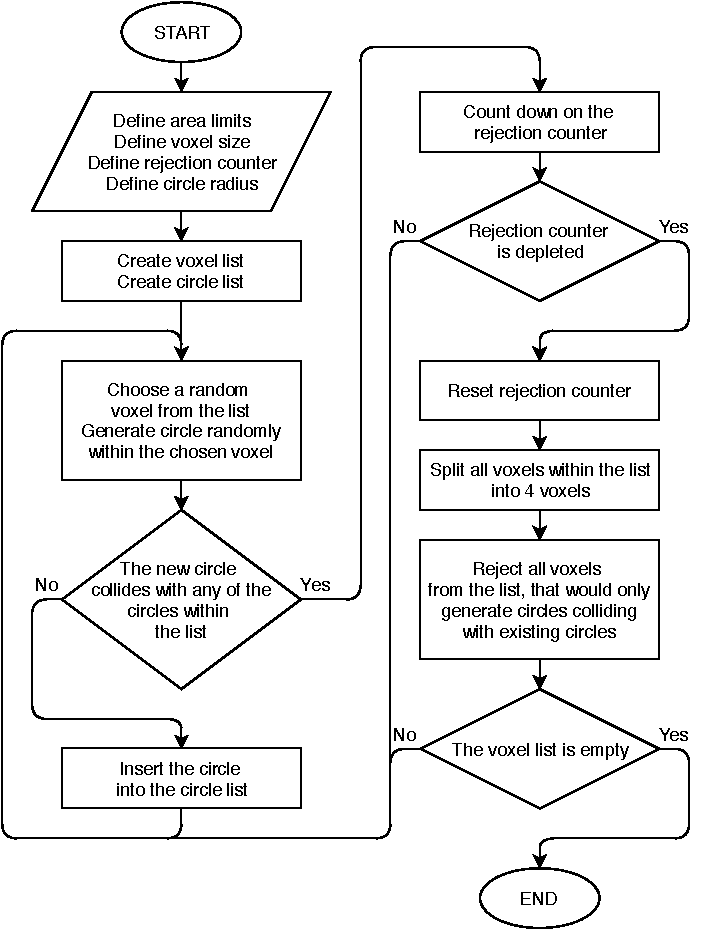
\includegraphics{Images/2dCircleRSA/VoxelCircleRSA.pdf}
  \caption{The flowchart of simple 2D RSA algorithm, using circles. \newline
		This algorithm can be expanded to remove voxels after every successful figure insertion, or to split voxels at a different condition.}

	\label{VoxelCircleRSApdff}
\end{figure}

\begin{figure}
  \centering

  \begin{subfigure}[b]{0.3\linewidth}
    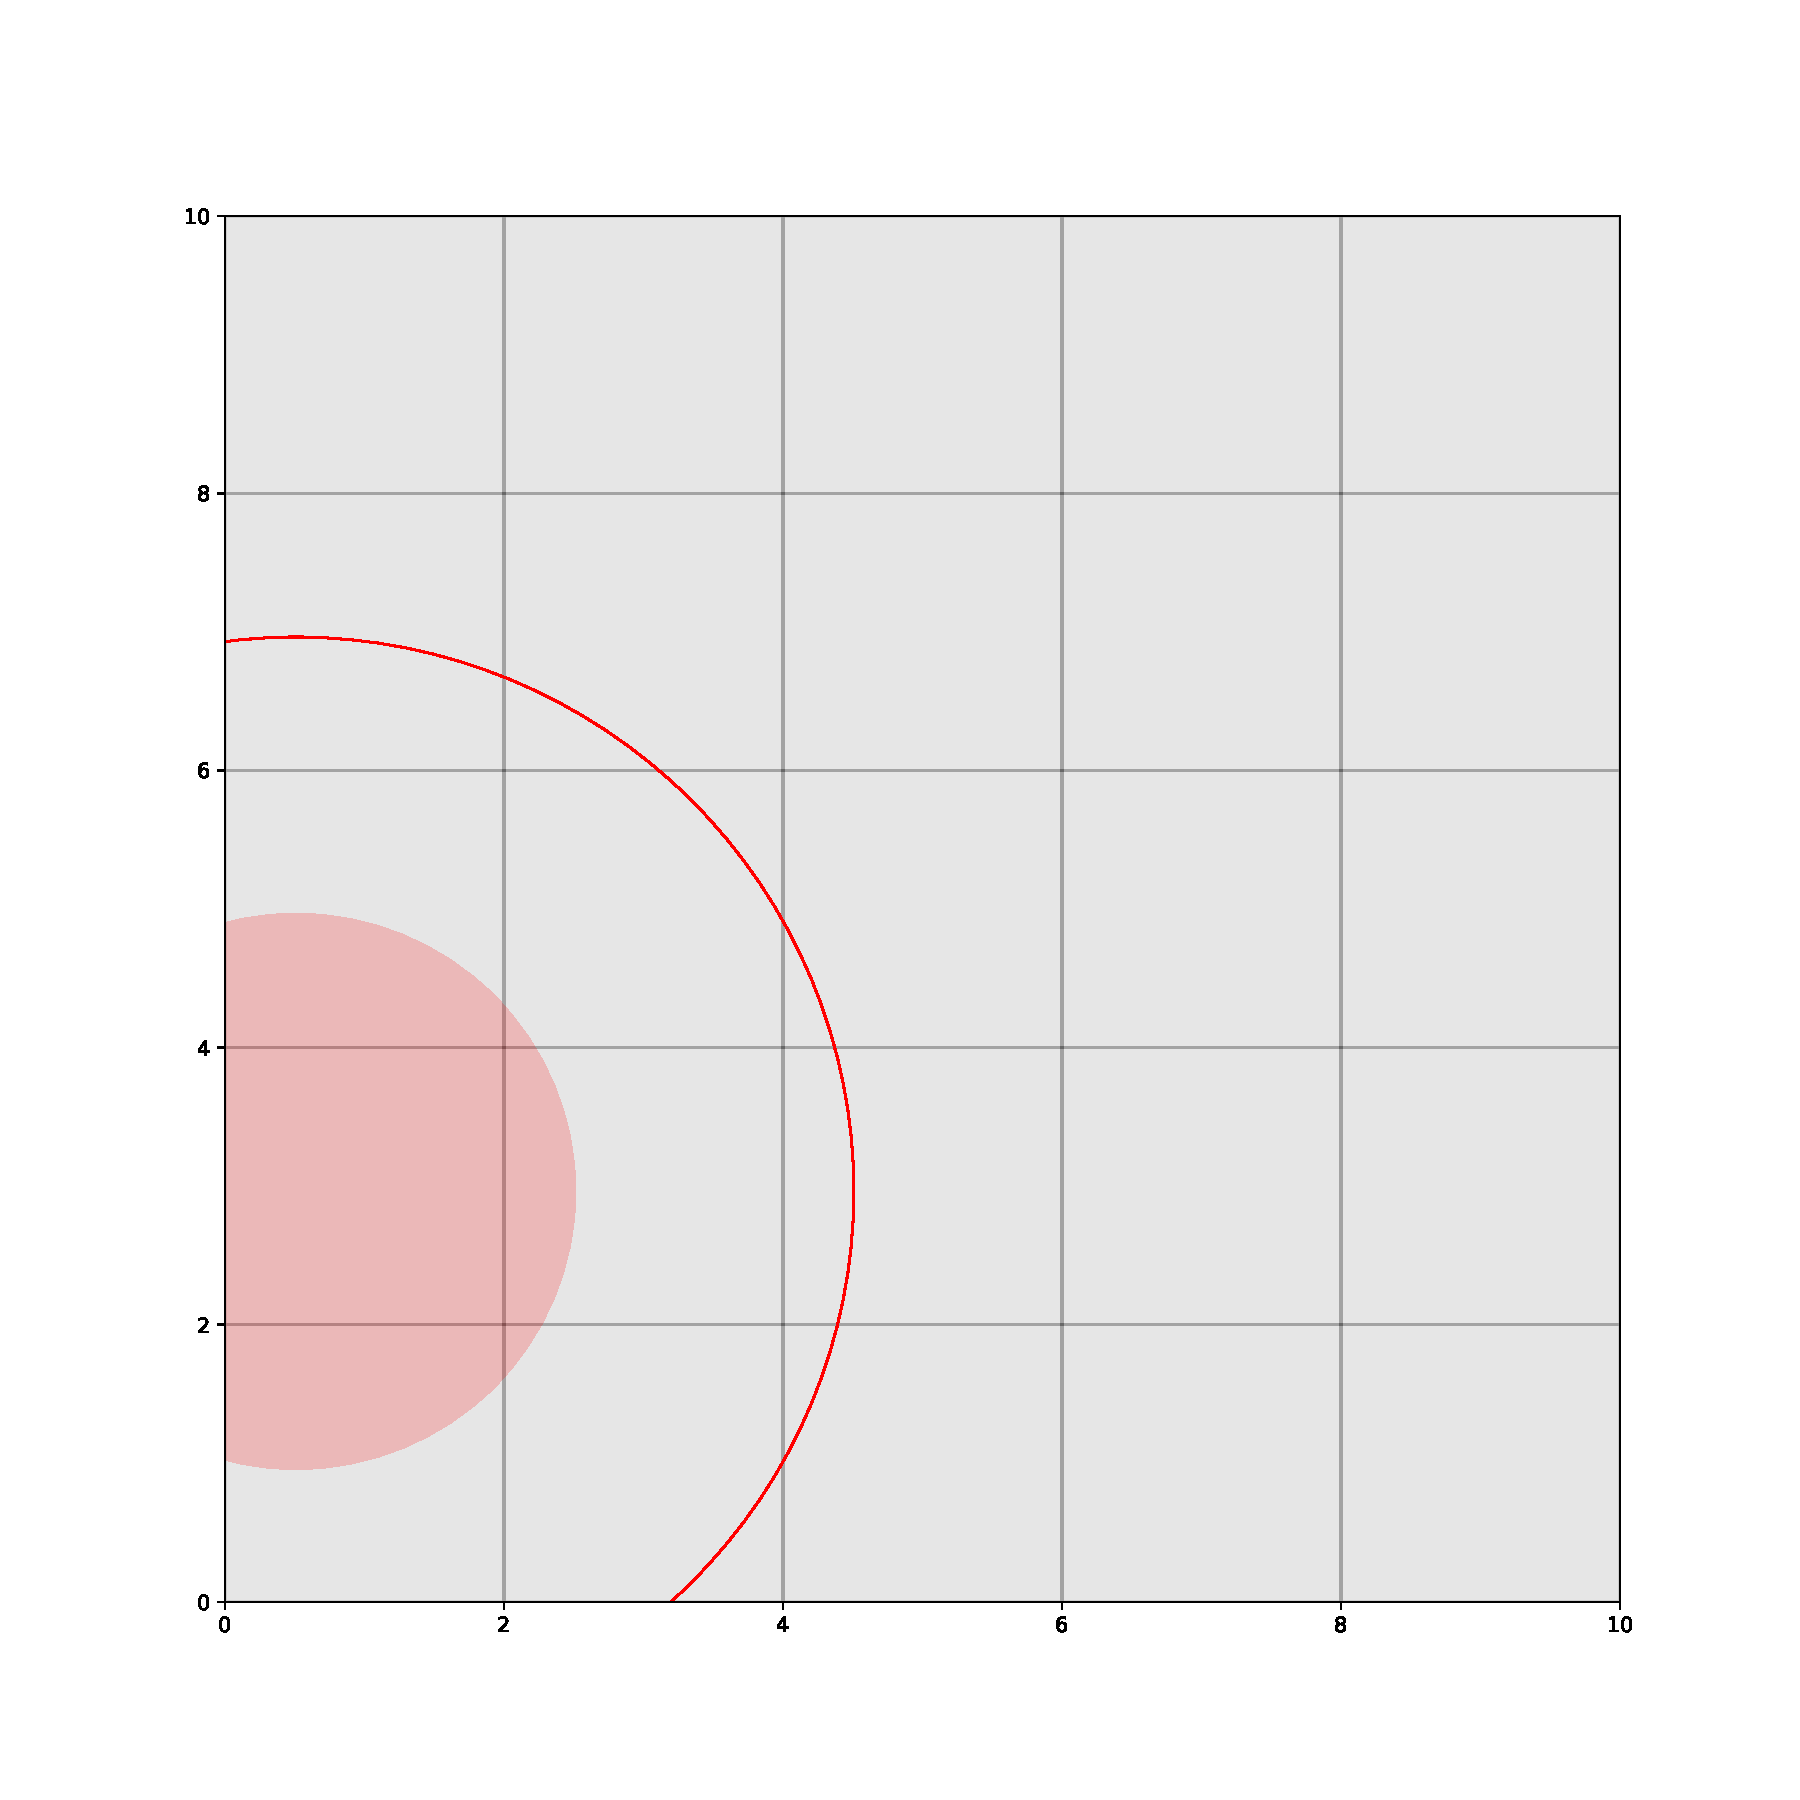
\includegraphics[width=\linewidth]{Images/2dCircleRSA/fig1.pdf}
    \caption{}
  \end{subfigure}
  \begin{subfigure}[b]{0.3\linewidth}
    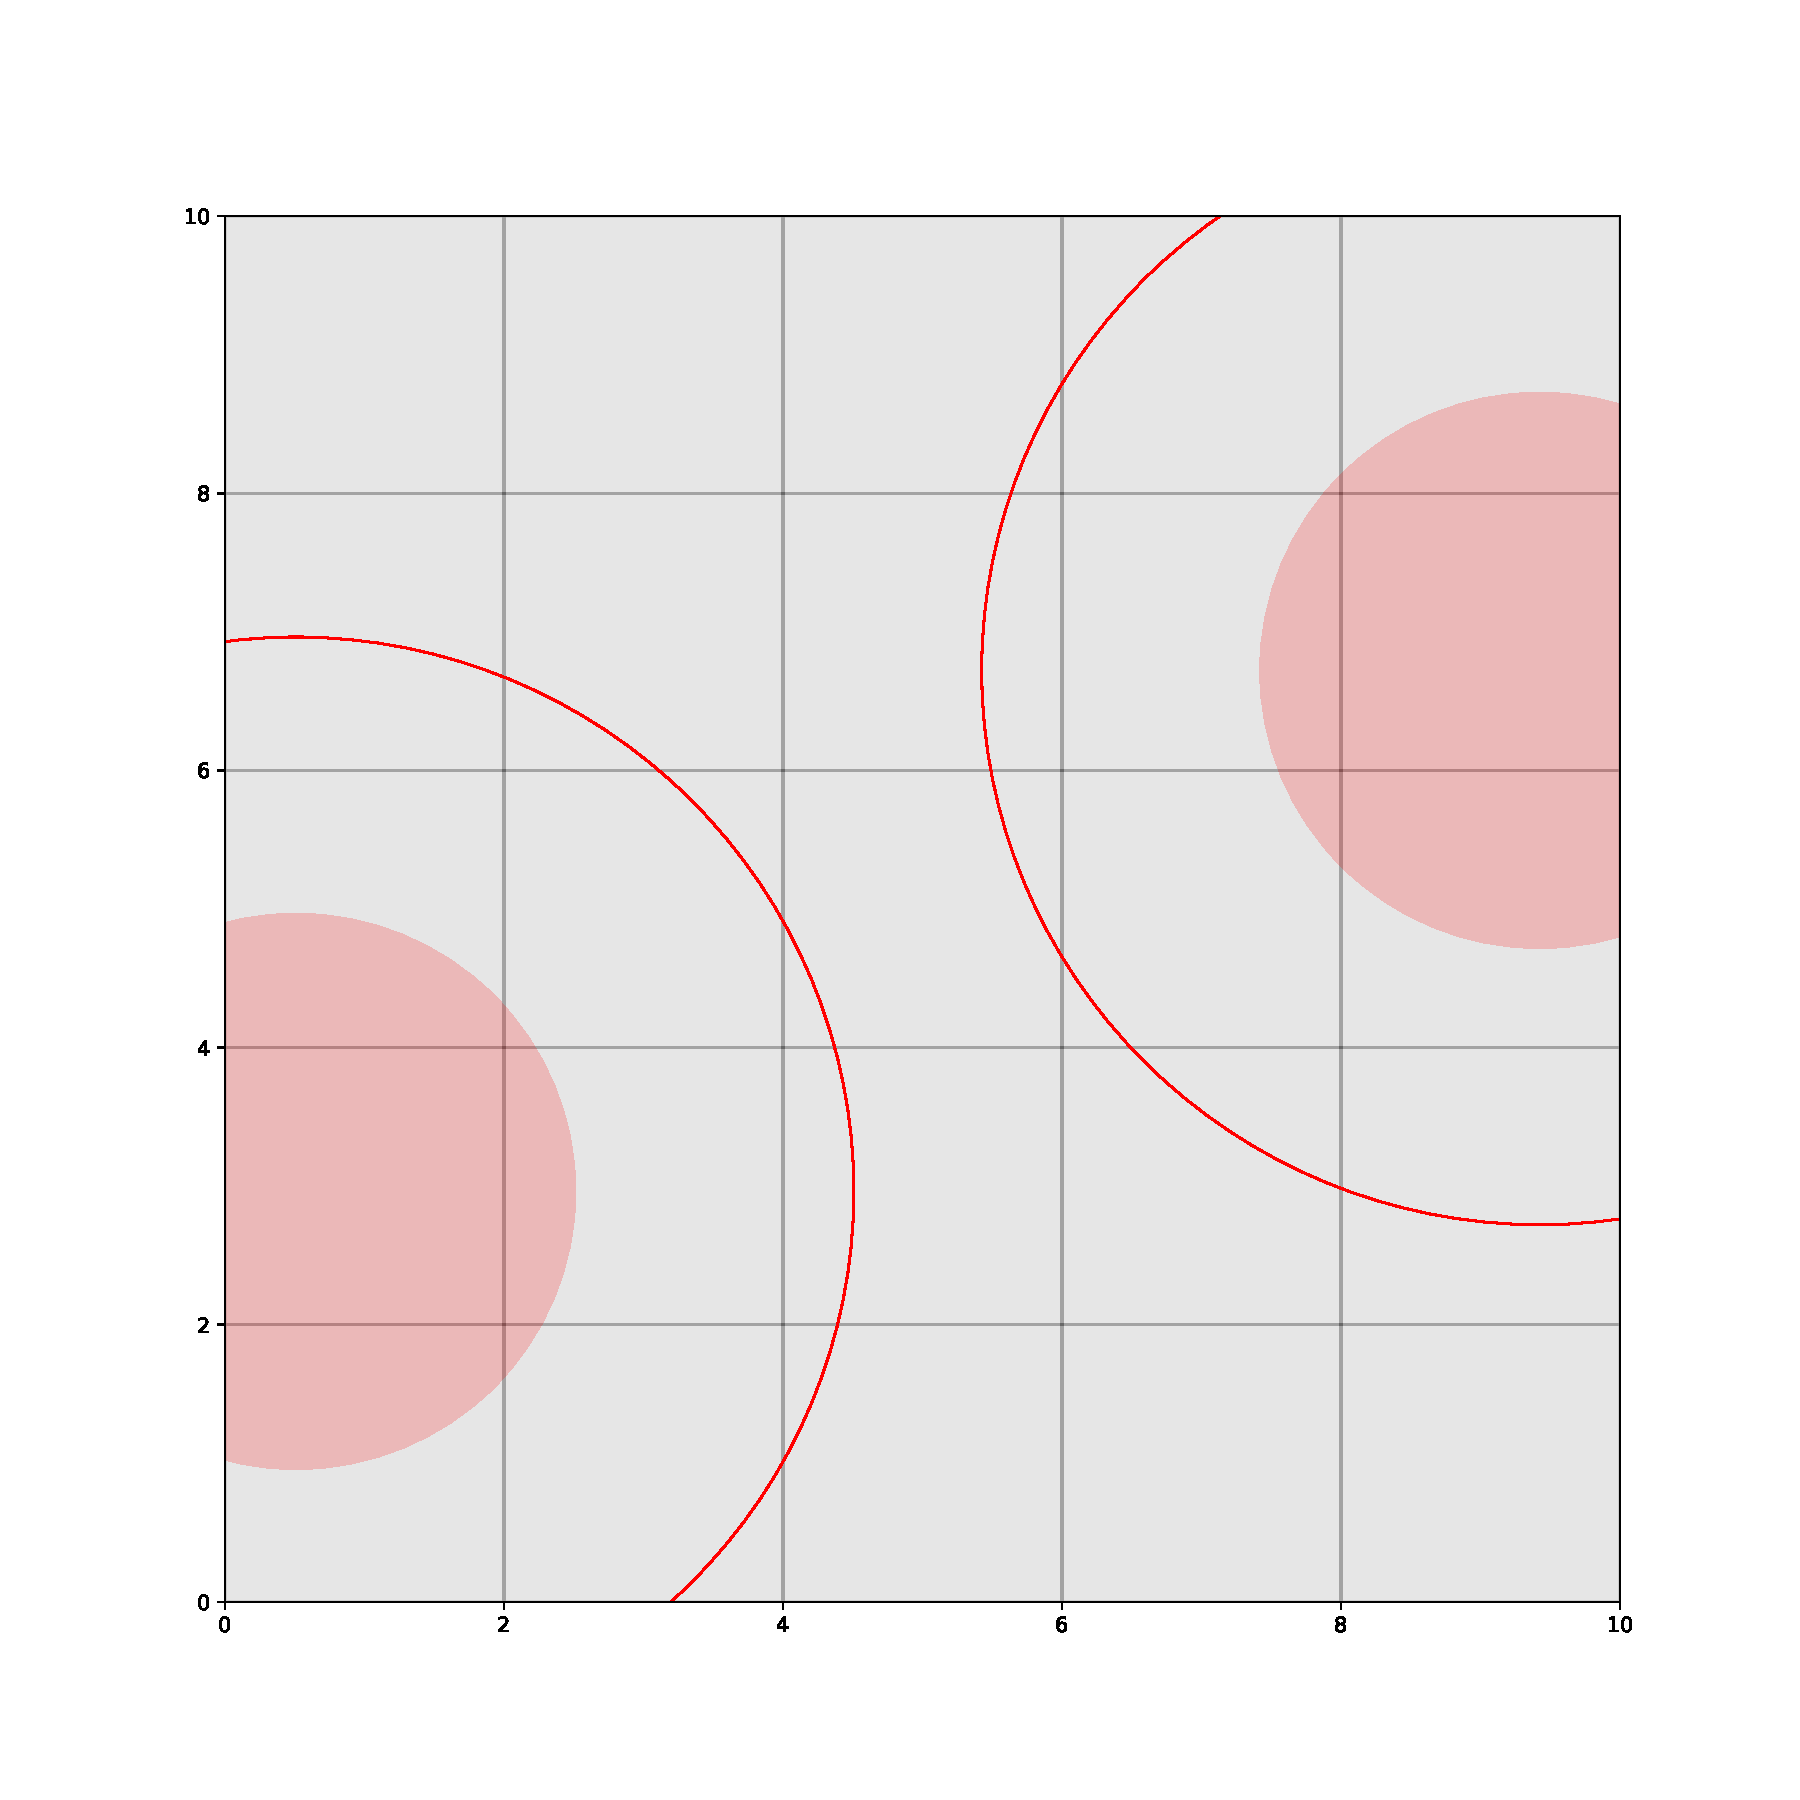
\includegraphics[width=\linewidth]{Images/2dCircleRSA/fig2.pdf}
    \caption{}
  \end{subfigure}
  \begin{subfigure}[b]{0.3\linewidth}
    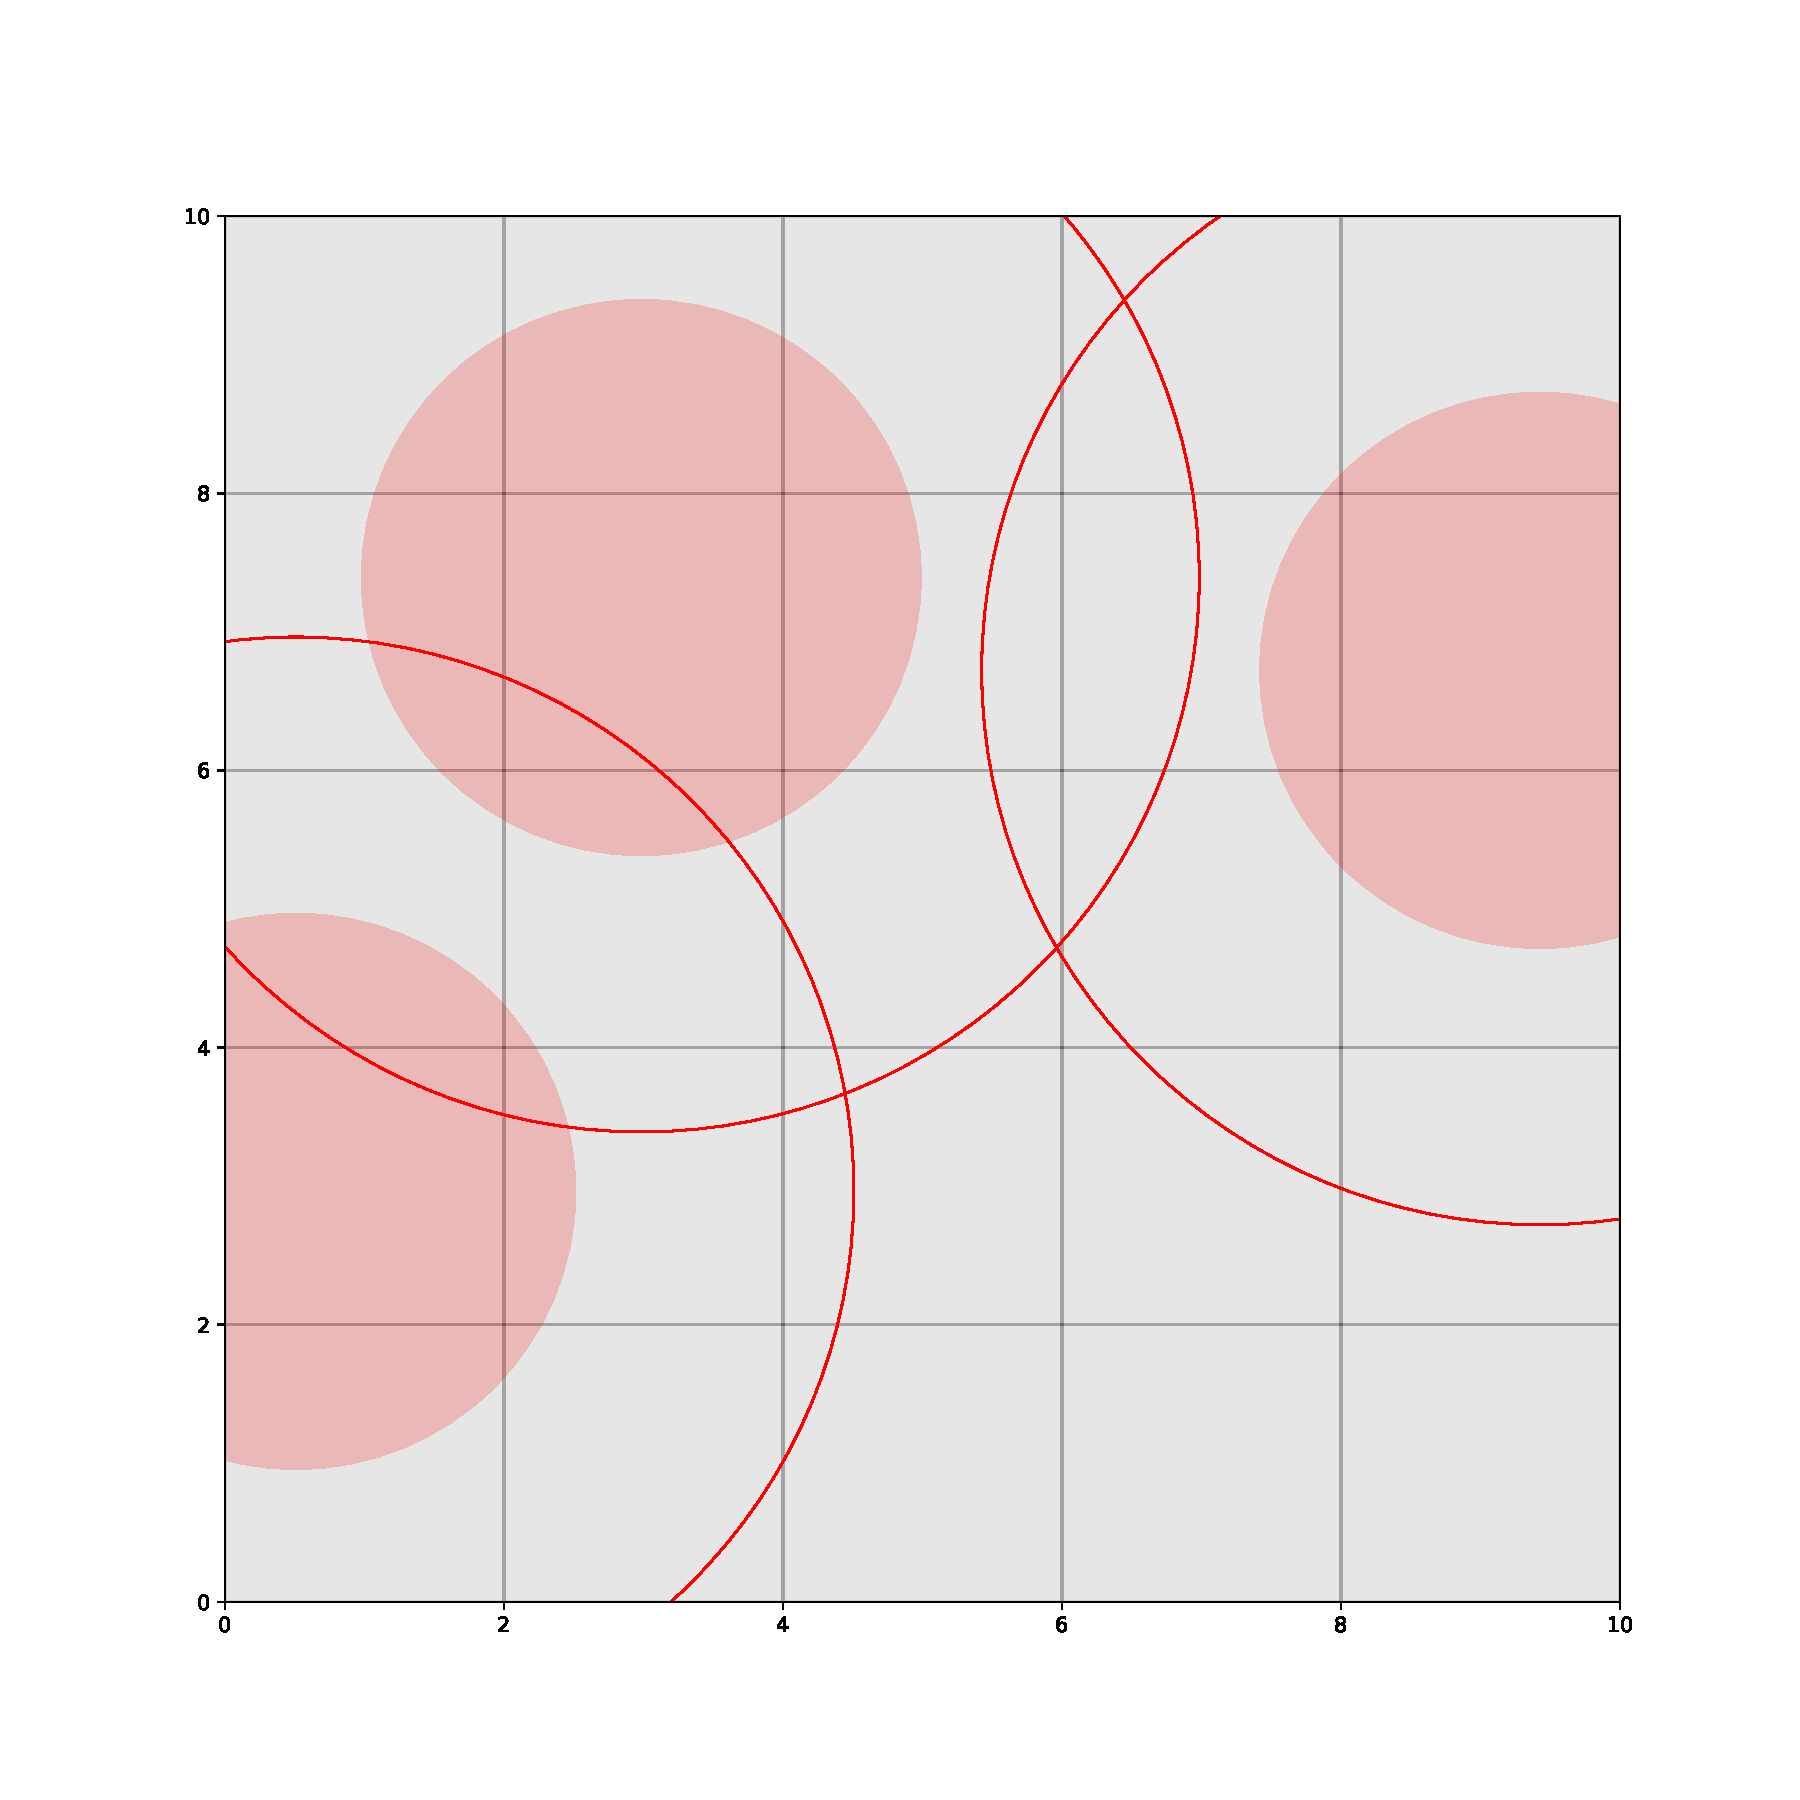
\includegraphics[width=\linewidth]{Images/2dCircleRSA/fig3.pdf}
    \caption{}
  \end{subfigure}

  \begin{subfigure}[b]{0.3\linewidth}
    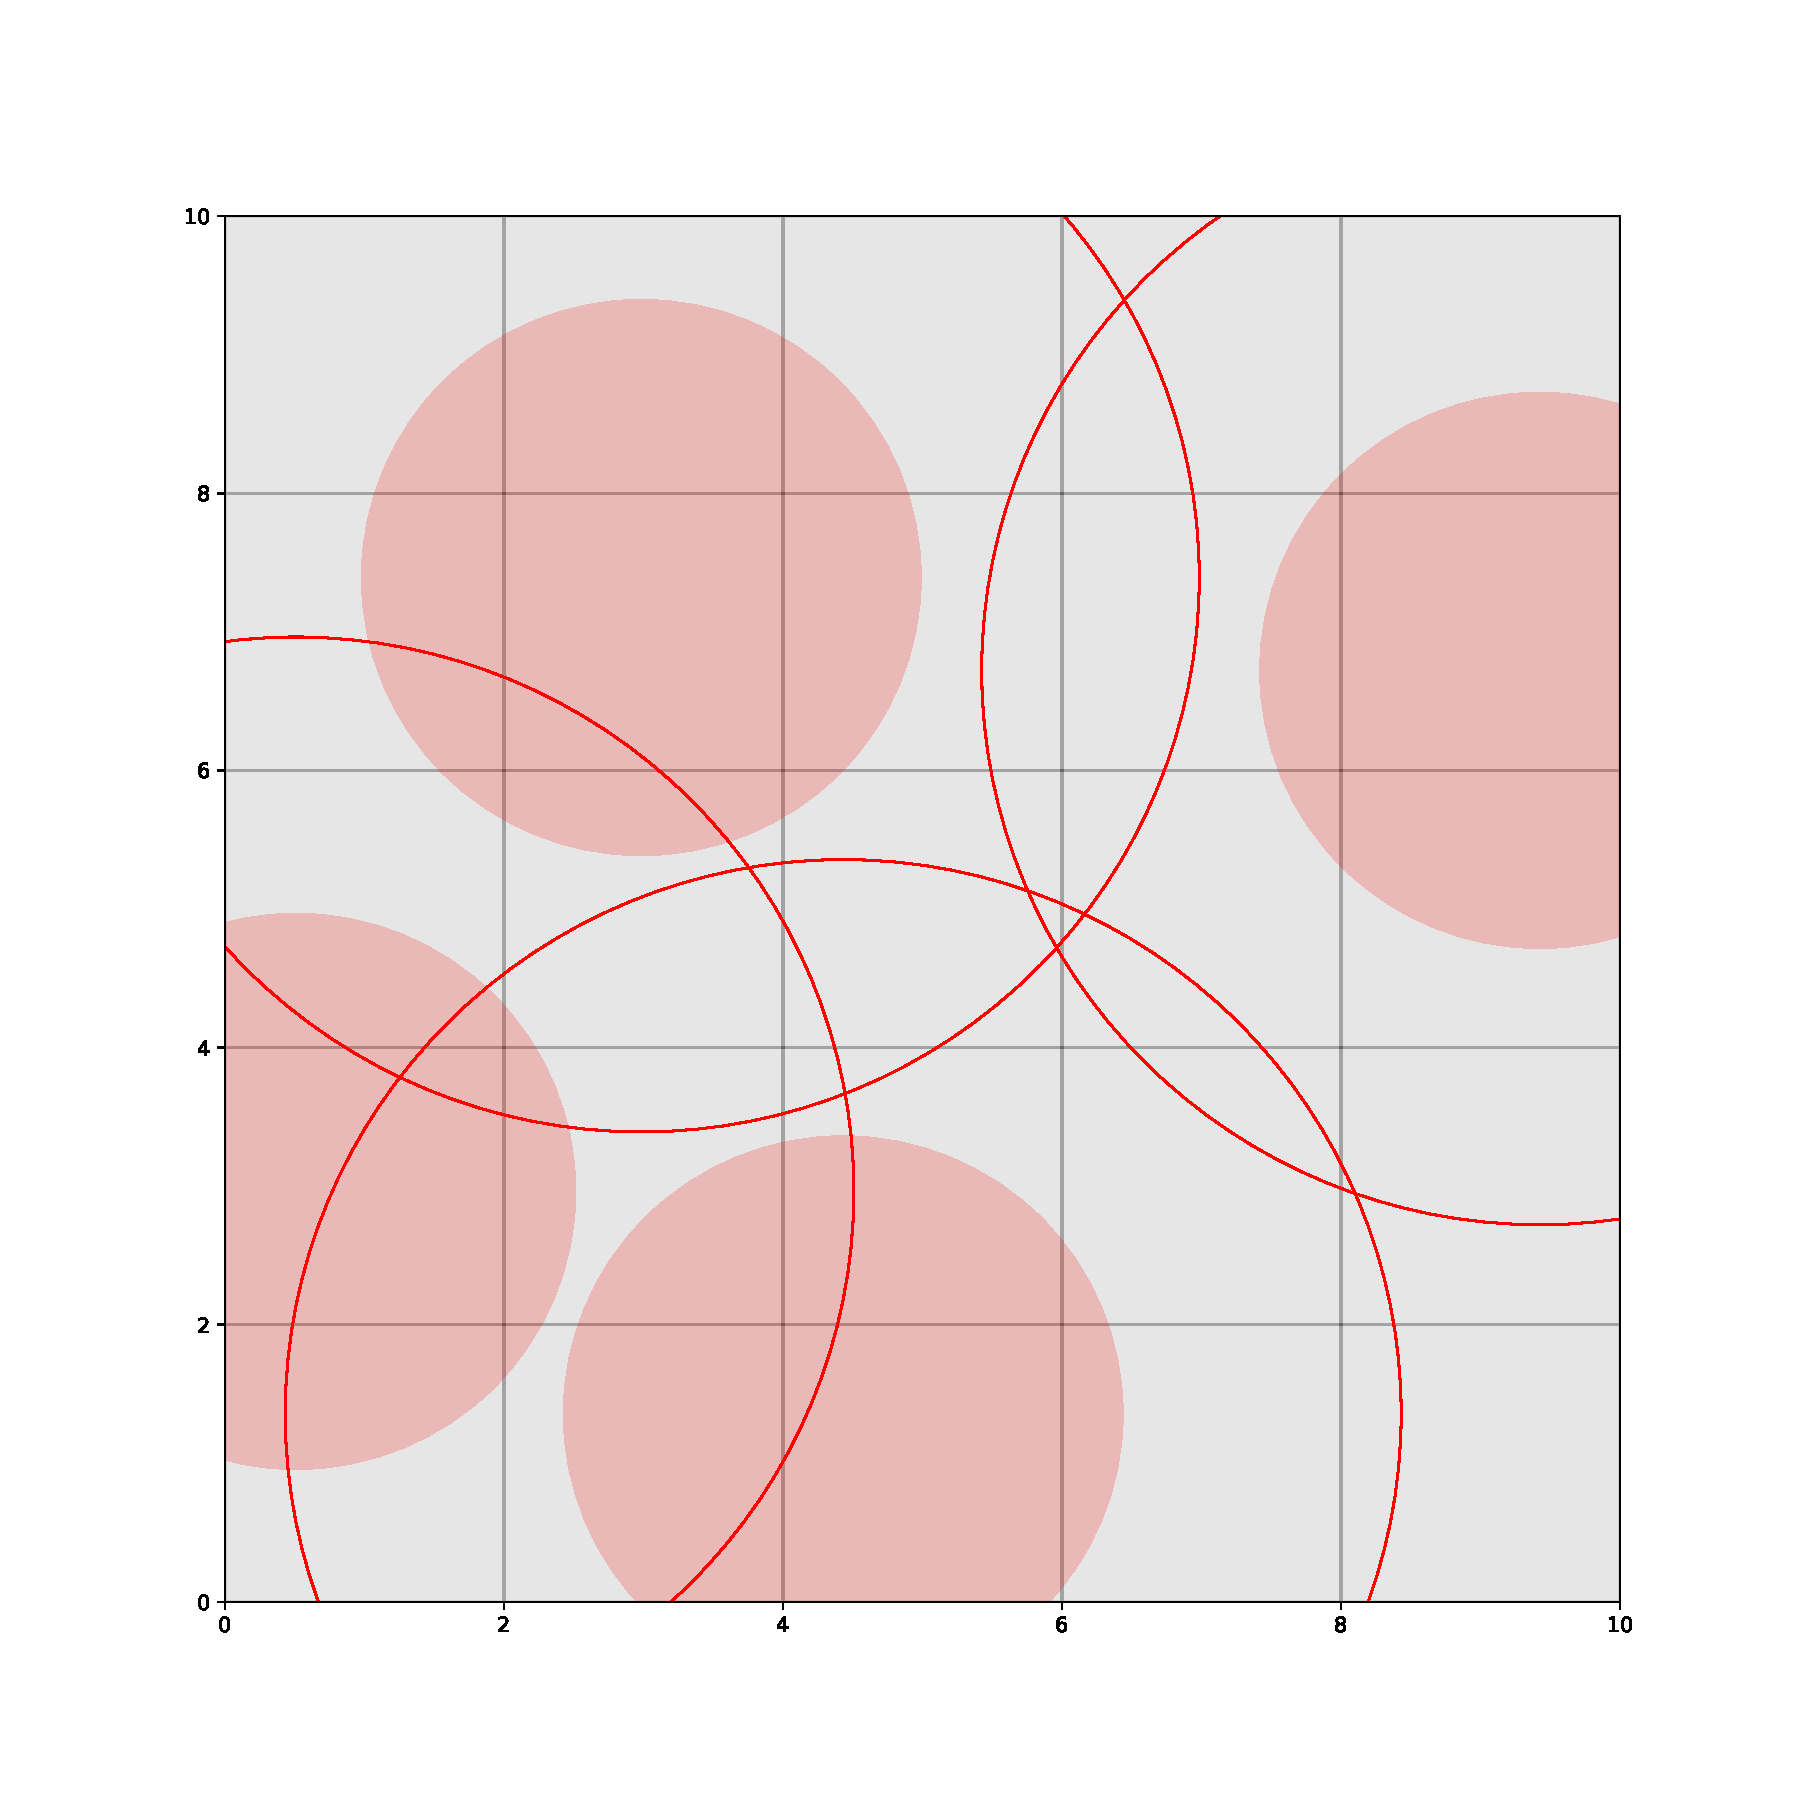
\includegraphics[width=\linewidth]{Images/2dCircleRSA/fig4.pdf}
    \caption{}
  \end{subfigure}
  \begin{subfigure}[b]{0.3\linewidth}
    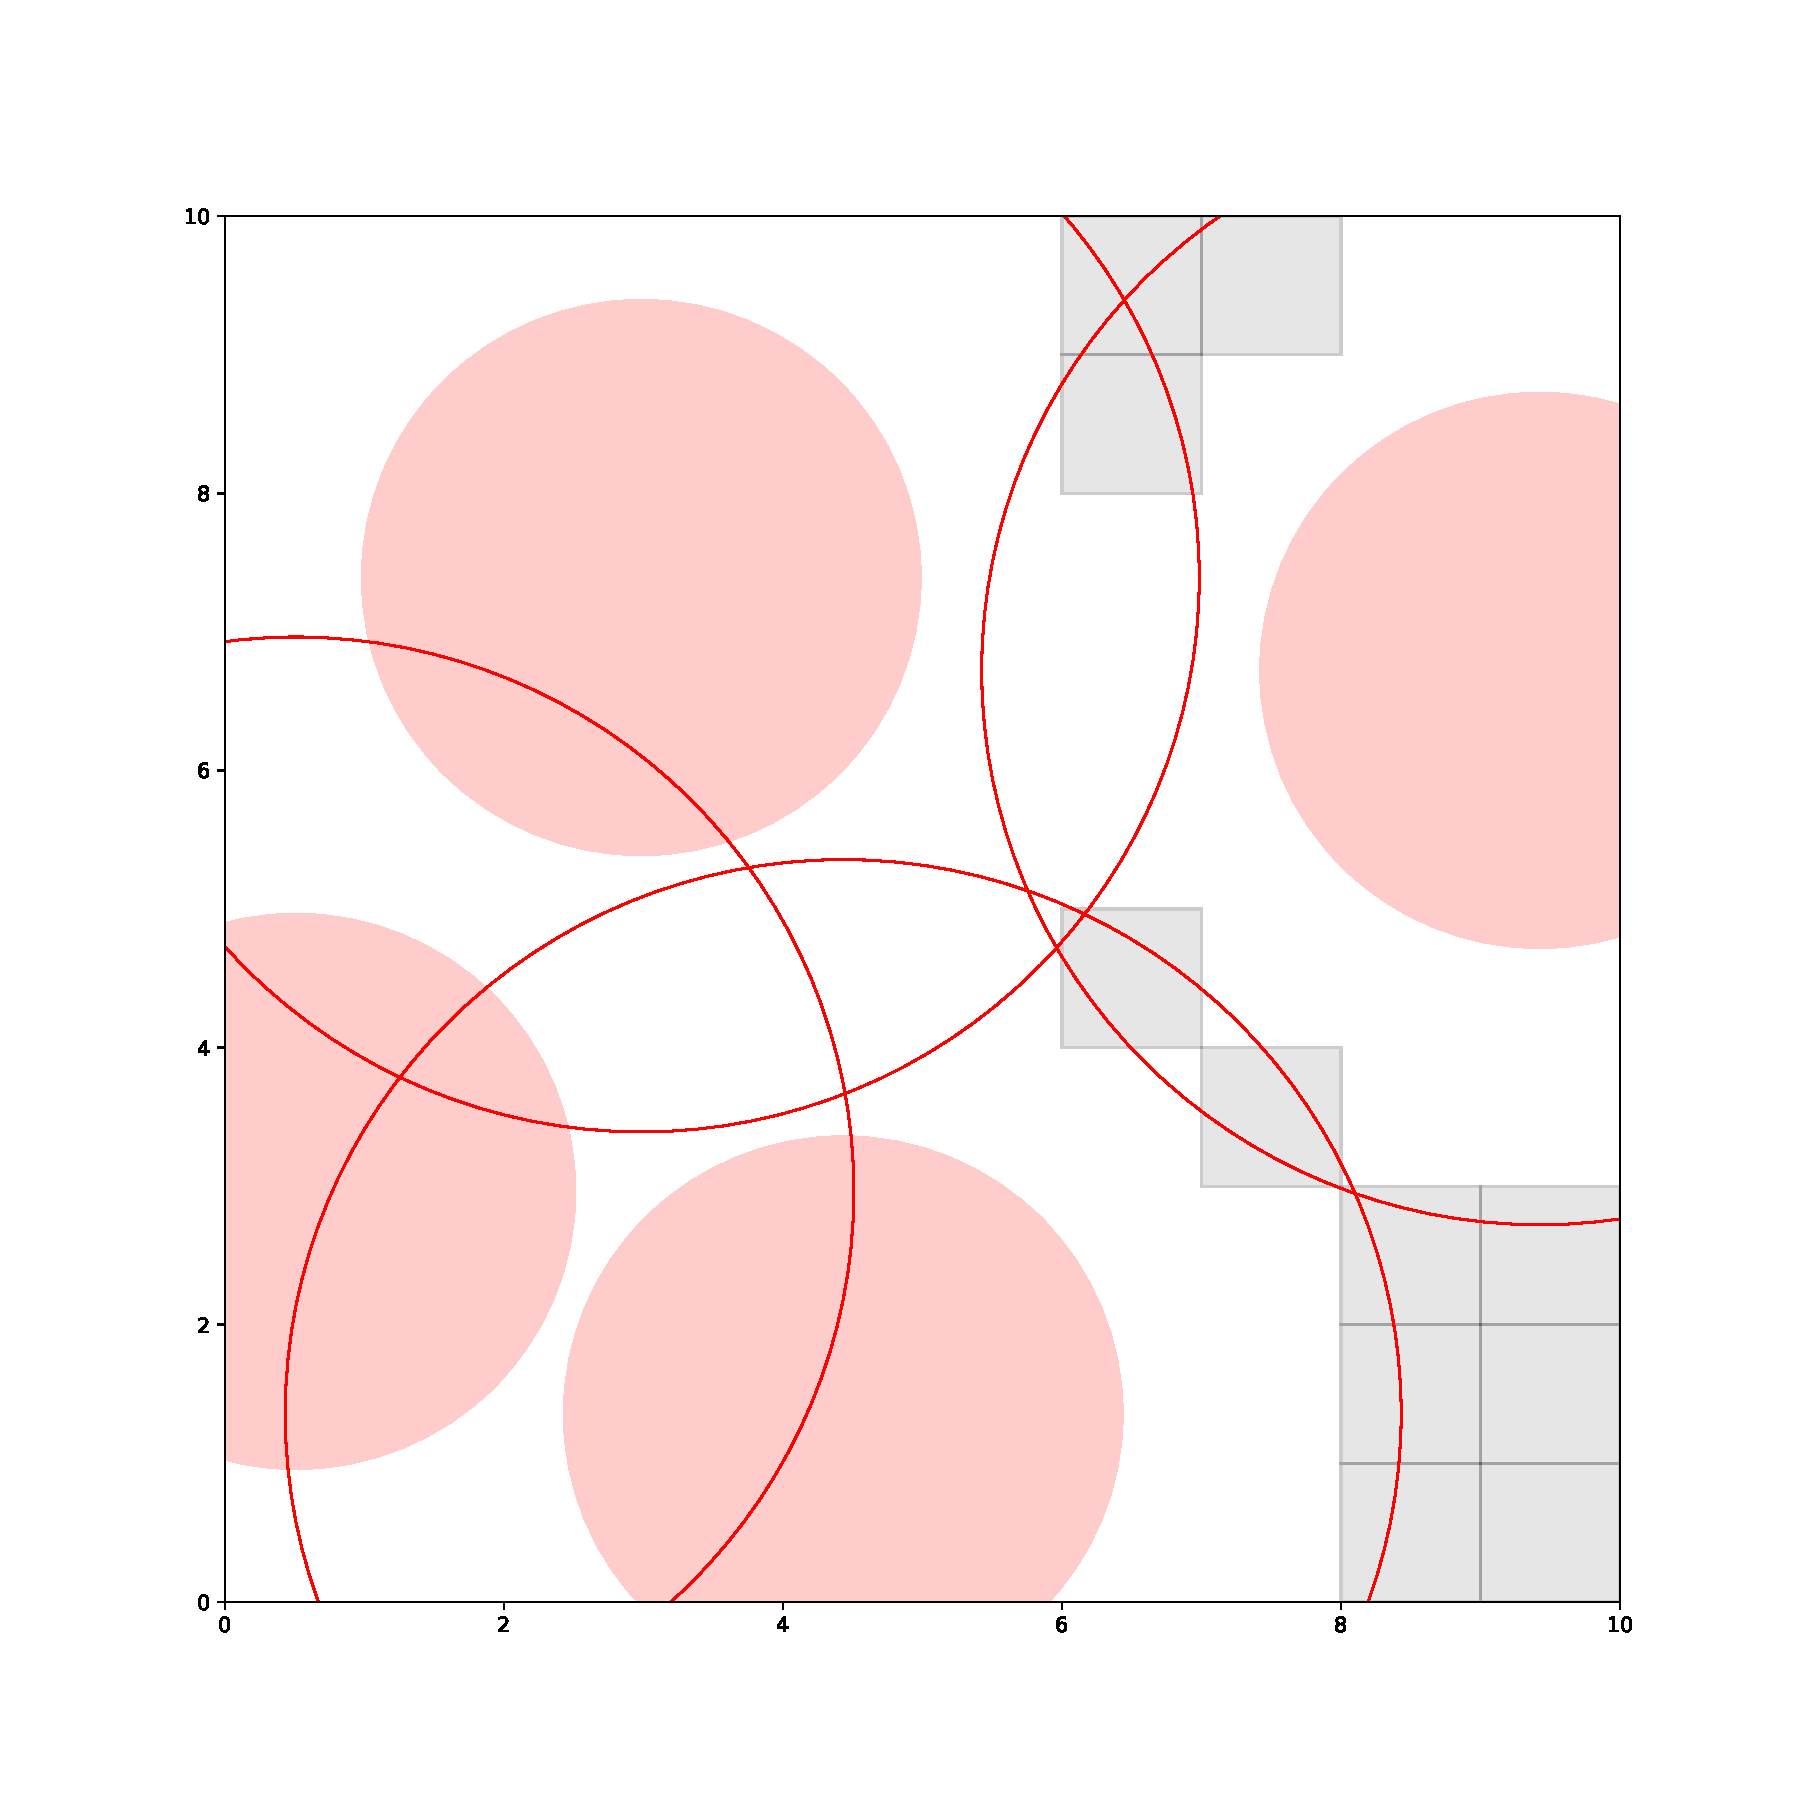
\includegraphics[width=\linewidth]{Images/2dCircleRSA/fig5.pdf}
    \caption{}
  \end{subfigure}
  \begin{subfigure}[b]{0.3\linewidth}
    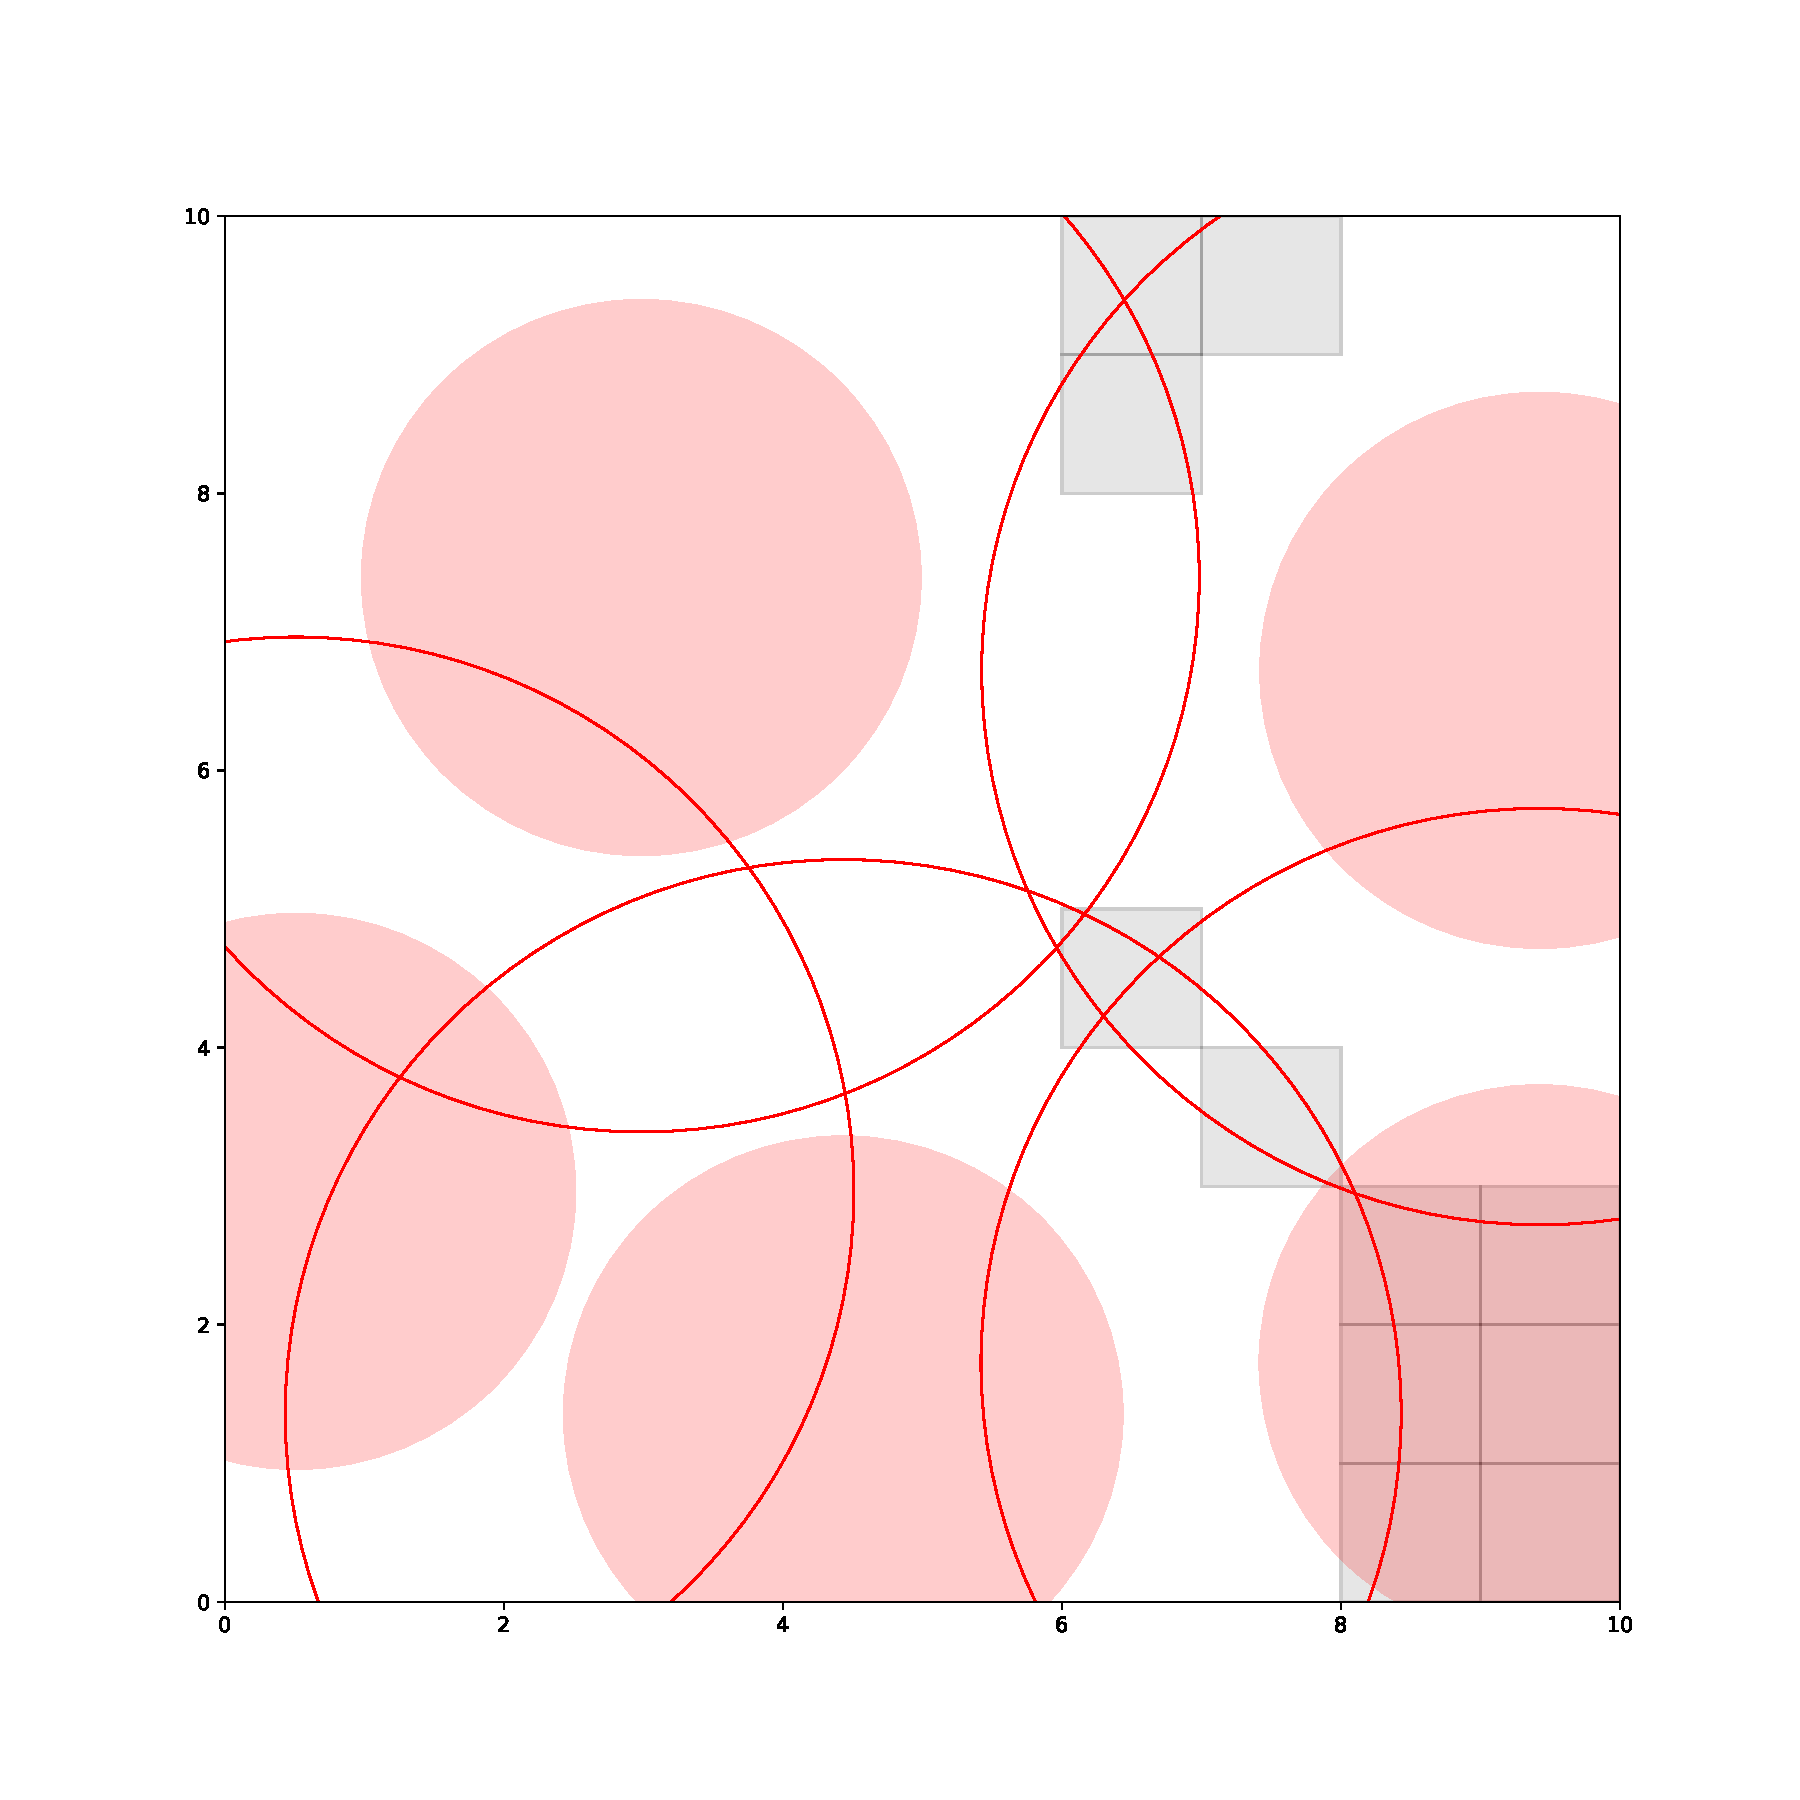
\includegraphics[width=\linewidth]{Images/2dCircleRSA/fig6.pdf}
    \caption{}
  \end{subfigure}

  \begin{subfigure}[b]{0.3\linewidth}
    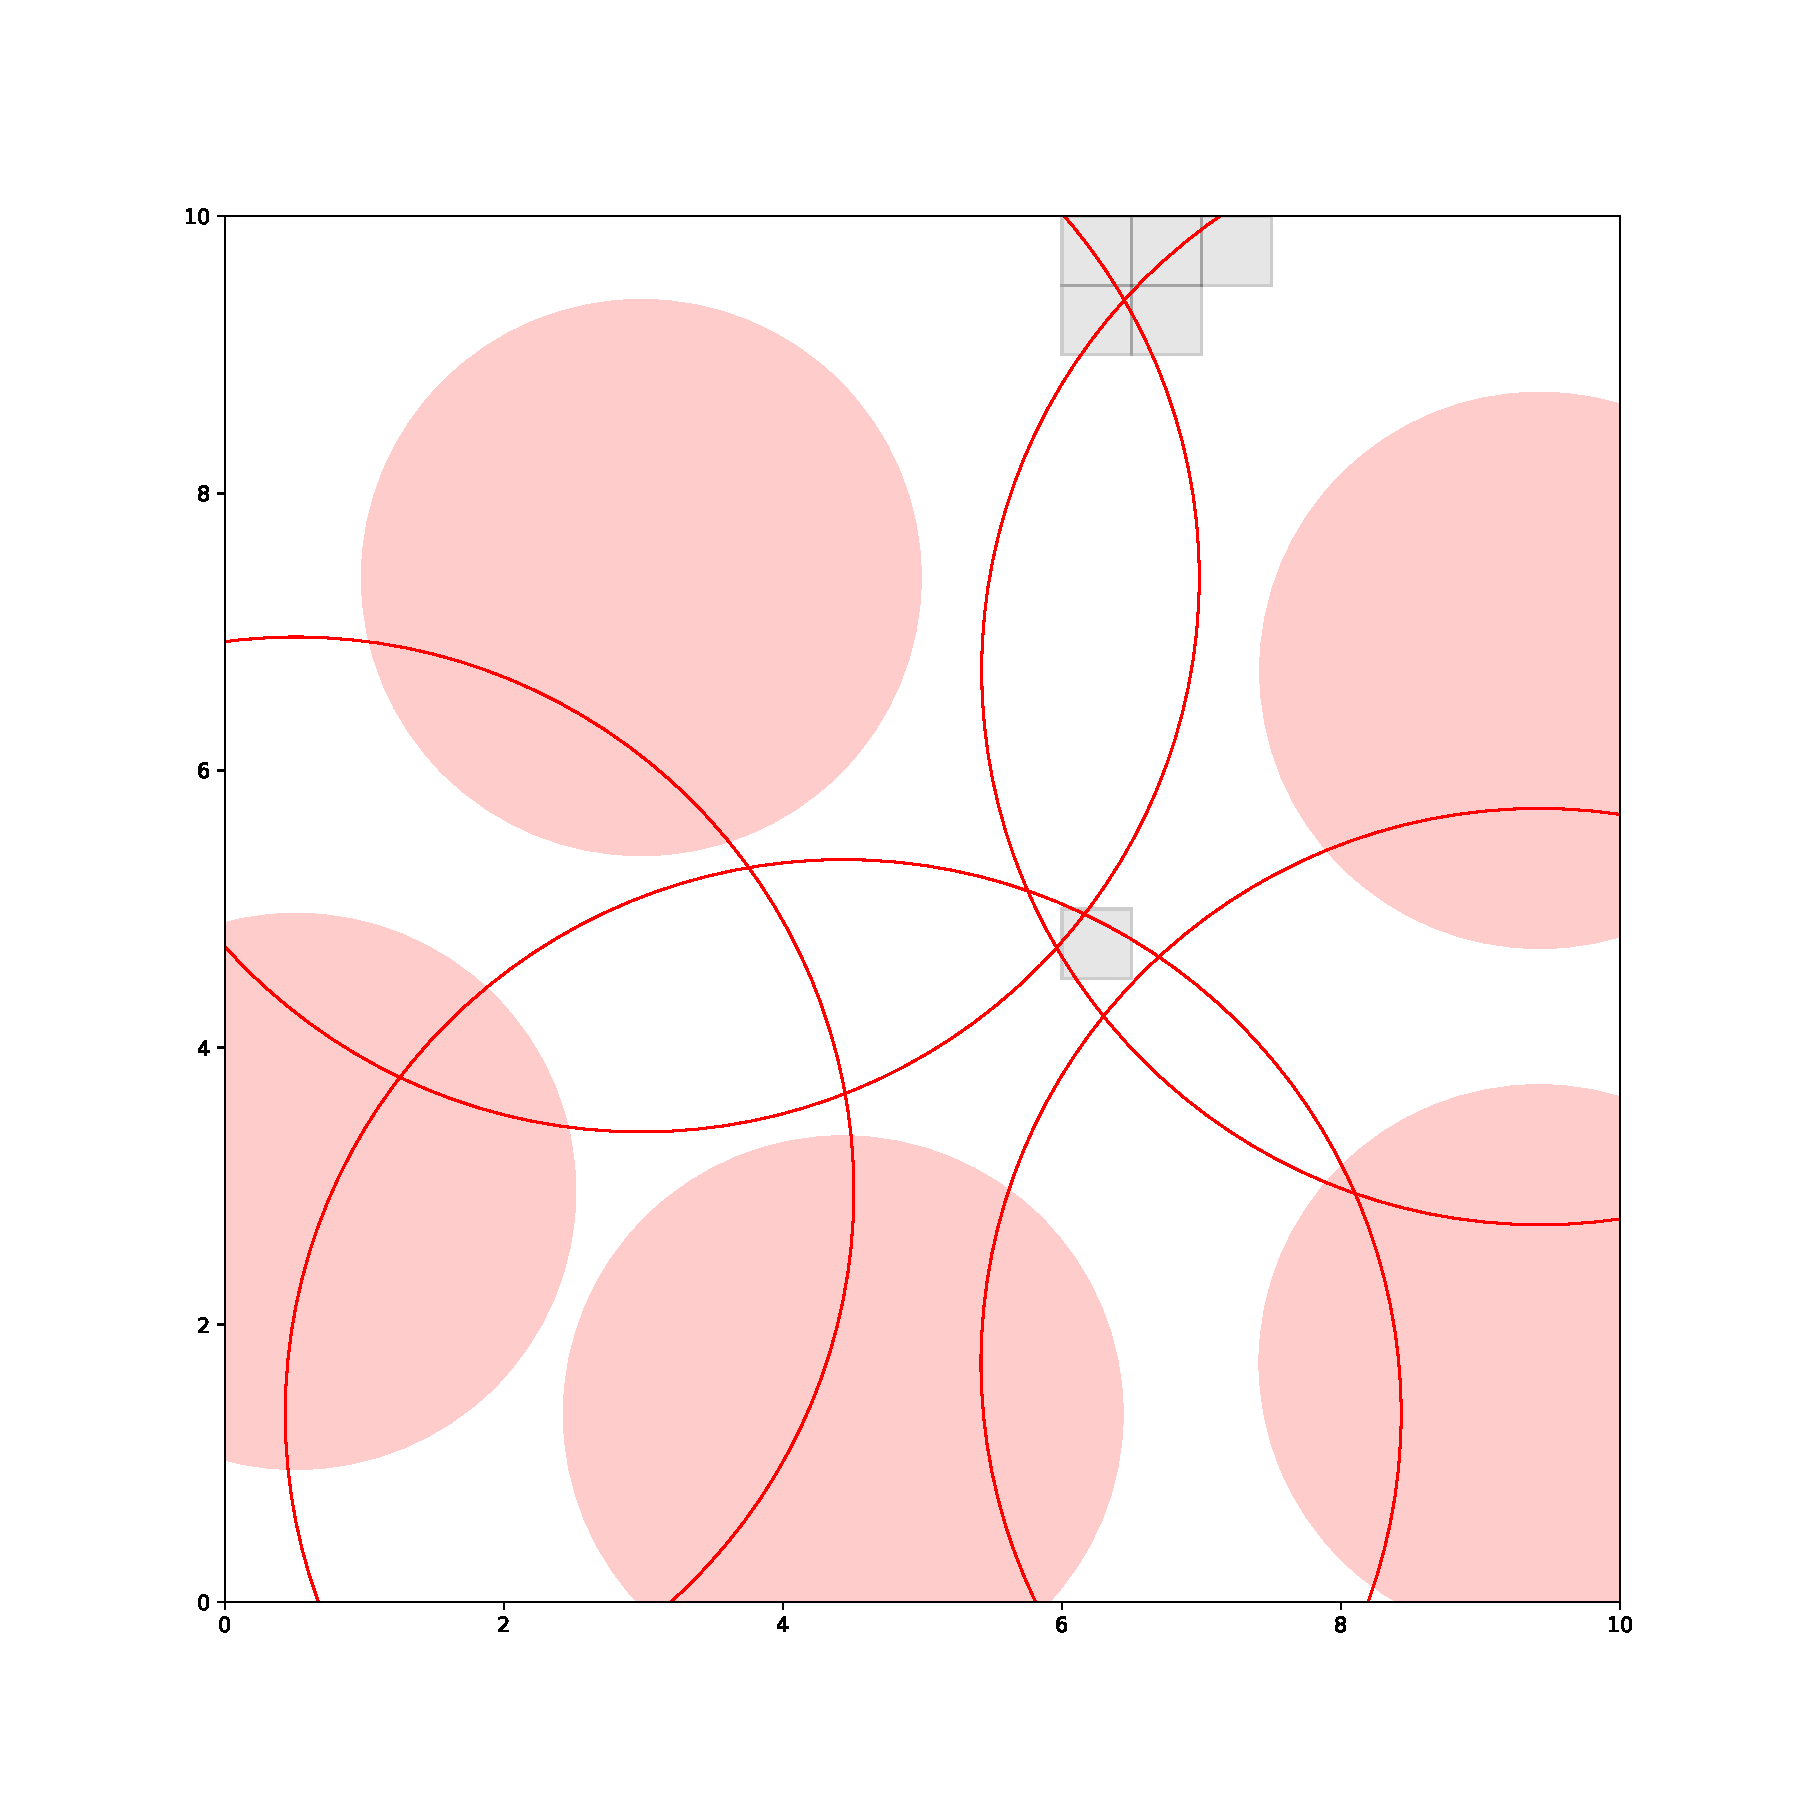
\includegraphics[width=\linewidth]{Images/2dCircleRSA/fig7.pdf}
    \caption{}
  \end{subfigure}
  \begin{subfigure}[b]{0.3\linewidth}
    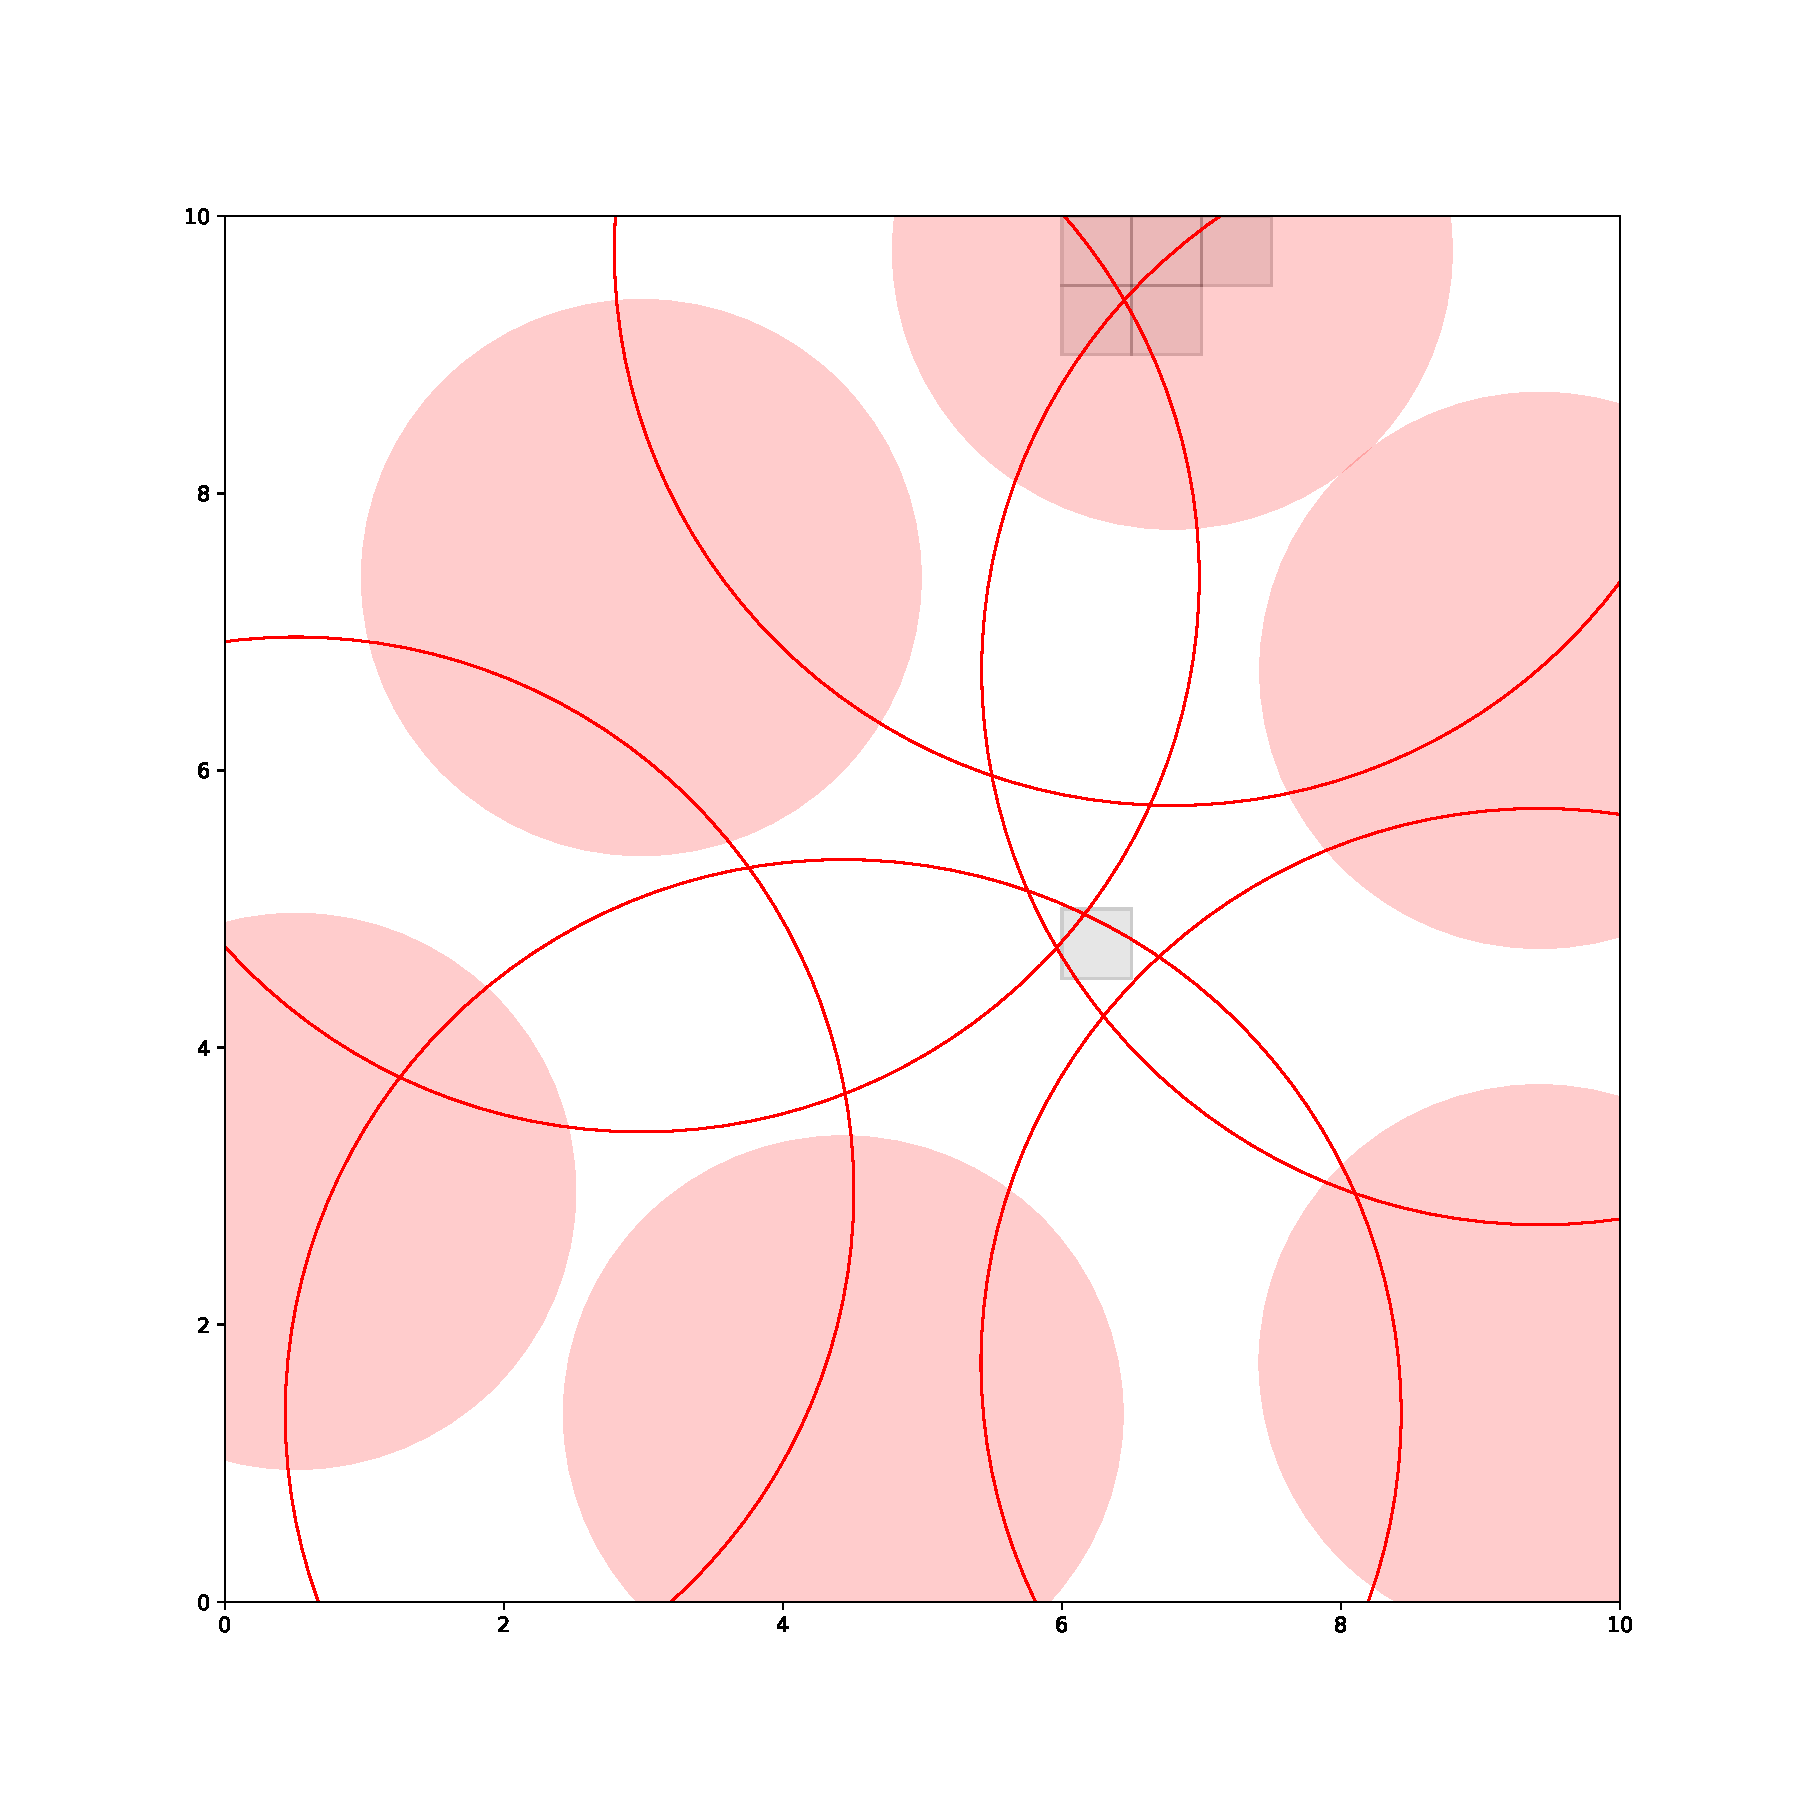
\includegraphics[width=\linewidth]{Images/2dCircleRSA/fig8.pdf}
    \caption{}
  \end{subfigure}
  \begin{subfigure}[b]{0.3\linewidth}
    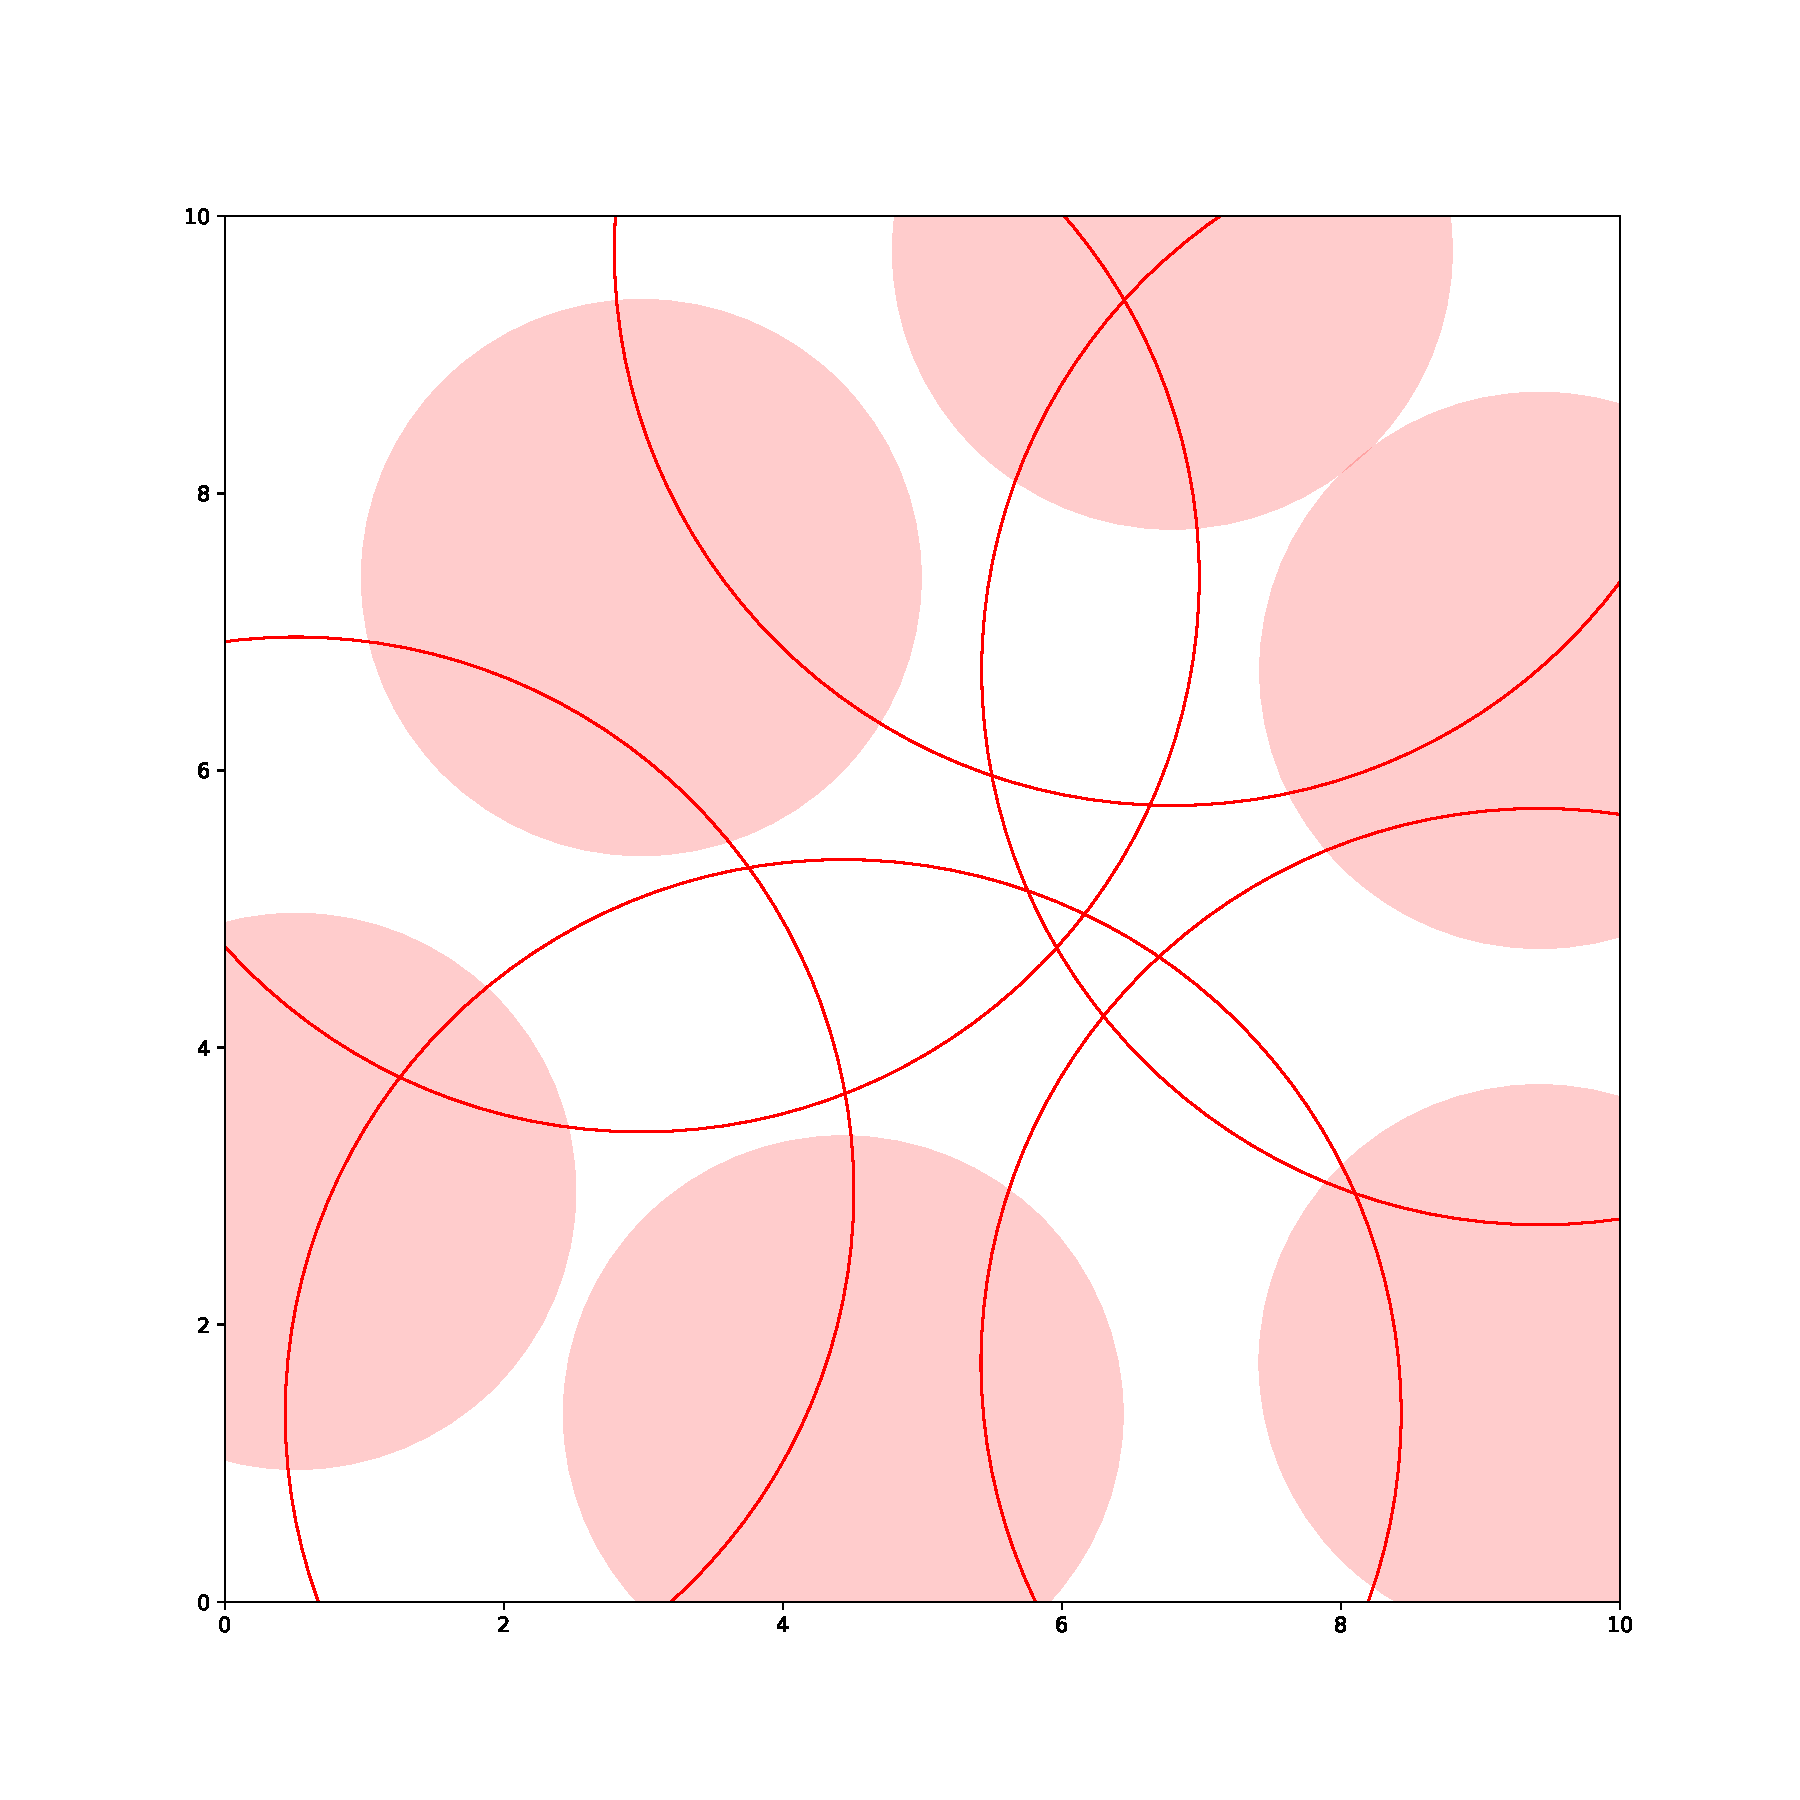
\includegraphics[width=\linewidth]{Images/2dCircleRSA/fig9.pdf}
    \caption{}
  \end{subfigure}

  \caption{This figures illustrate a simple run of the described simple 2D RSA algorithm. \newline
		World size is 10.0 by 10.0, the inserted circles have the radius of 2.0. The initial voxel side has length of 2.0. After 10 failed attempts at inserting the circle, the voxels are subdivied and rejected.\newline
		The figures \textit{a,b,c,d} show the insertion of the first four circles. The figure \textit{d} illustrates the effect of the voxel subdivision and rejection. Following figures illustrate next iterations of circle insertions, voxel subdivisions and removals, and finally, at figure \textit{i}, completely saturated system with no remaining voxels. \newline
		The voxels are rejected if they lie entirely within the double radius of any circle - in such case any circle generated within the voxel would collide with the evaluated circle. This is determined by examining if distance to all vertices of a voxel is less than the circle's doubled radius. This doubled radius is marked here as a solid red outline.}
  \label{VoxelCircleRSApdfExamples}
\end{figure}


\section {Sequential Algorithm}

The algorithm developed by dr. hab. Cieśla is an expansion on the previusly described basic model. However, some changes have been made to accomodate the algorithm to a different shape, more efficient execution and a modification in the behavior of space.

\subsection{Periodical Edge Conditions}

The algorithm was supposed to operate using a space that, unlike previously shown model, would \textit{loop} at the edges. This means, that if a shape is placed nearby the edge of given space, the shapes placed at the opposite edge of the space collide with it. They behave as if the opposite edge of the space would be a continuation of this edge. The periodical edge conditions serve to improve packing efficiency, and remove edge-related artifacts. In essence, the periodical edge conditions 'simulate' an infinite area, and thus may be helpful to model surfaces of far greater area than the provided space.\autocite[1]{ciesla_mziff}

\subsection{Adjacency Matrix}

During the execution of the algorithm, there are two places where a function must be performed at two objects, many different times. Firs, when the shape is inserted, it is determined if it collides with any other existing shape. The other time, it is when the voxel is rejected - it must be checked against all shapes, until one that would cause it's rejection is found. It is possible to limit the executions of these function to a far lesser number; By dividing the world into a number of cells, with sides as long as the radius of the shape's minimum binding circle, it is only nescessary to check the collisions of the shapes that belong to the same, or neighboring cells (similarly with voxels). This limits the number of collision checks that need to be performed to a theoretical maximum, based on how many shapes can fit into a three-by-three cell neighborhood. \newline
This solution can also be helpful with the periodical edge conditions problem. Having a quick access to the cell given it's coordinates enables the program to easily reference shapes from the opposite edge, by tapping into the target cell and translating the shapes stored by it.

\subsection{Polydisk Collision}

Since the algorithm uses a shape consisting of a list of disks with given radiuses and a relative position to an arbitrary center, it is relatively easy to check if two such shapes collide. It is enough to loop over both lists of shapes' circles absolute positions, checking if any two collide. \newline
The much more complex problem is the voxel rejection. The first problem is that since the shapes can have a different angle, this needs to be implemented in the voxels structure - the solution was to add a third dimension, representing the available angles in which the shapes may appear.

\textbr{UNFINSHED - ASK HOW THIS WORKS, HOW TO DESCRIBE IT}


\section {Parallel Application}

Having the available algorithm for sequential execution, the main challenge consisted of modifying it to enable a highly parallel execution using the GPU. The modified algorithm executes some parts of the problem sequentially, as it was not possible to parallelize it entirely.

\subsection{Block Graph}
	%draw a block graph
\section {Implementation}
	%write in general about implementing, challenges etc
\subsection{PyCuda}
	%write about language specifics, improvements over raw CUDA
\subsection{Visualisation}
	%about pyplot - shortly
\subsection{Summary}
	%stuff in general

{\bf TODO unfinished, do in near future}

%ACTUAL THESIS: RESULTS INVESTIGATION ====================================================

%15-25 pages - due to multiple pictures
\chapter{Results Examination}
\section{Performance Evaluation}
	%describe importance of performance evaluation
	%describe the algorithm runner, and hot it works
\subsection{Parameter Influence over Performance}
\subsection{Shape Influence over Performance}
{\bf TODO unfinished, do later}

%ACTUAL THESIS: BIBLIOGRAPHY ====================================================

\newpage
\printbibliography

\end{document}
